
\documentclass[preprint2]{emulateapj}

\usepackage{natbib}
\bibliographystyle{apj}
\usepackage{longtable}
\usepackage[]{graphicx}
\usepackage{amsmath}
\usepackage{natbib}
\usepackage{tabularx}
\usepackage{bm}
\usepackage{color}

%% Sometimes a paper's abstract is too long to fit on the
%% title page in preprint2 mode. When that is the case,
%% use the longabstract style option.

%% \documentclass[preprint2,longabstract]{aastex}

\newcommand{\vdag}{(v)^\dagger}
\newcommand{\myemail}{gsavorgn@astro.swin.edu.au}
\newcommand{\fitfigurewidth}{0.8\textwidth}


\shorttitle{M-M paper}
\shortauthors{Savorgnan et al.}

\begin{document}

\title{Supermassive black holes and host bulges affairs -- \\ II. The red and the blue sequences in the mass -- mass diagram.}

%\author{G. A. D. Savorgnan\altaffilmark{1} and A. W. Graham\altaffilmark{1} and A. Marconi and E. Sani\altaffilmark{3} and L.K. Hunt}
%\affil{Centre for Astrophysics and Supercomputing, Swinburne University of Technology, Hawthorn, Victoria 3122, Australia.}
%\email{gsavorgn@astro.swin.edu.au}


\author{G. A. D. Savorgnan and A. W. Graham}
\affil{Centre for Astrophysics and Supercomputing, Swinburne University of Technology, Hawthorn, Victoria 3122, Australia.}
\email{gsavorgn@astro.swin.edu.au}
\author{A. Marconi}
\affil{?}
\author{E. Sani}
\affil{European Southern Observatory, Alonso de Cordova, Vitacura 3107, Santiago, Chile.}
\and
\author{L.K. Hunt}
\affil{?}

%\and

%\author{A. W. Graham\altaffilmark{1}}
%\affil{Centre for Astrophysics and Supercomputing, Swinburne University of Technology, Hawthorn, Victoria 3122, Australia.}

%% Notice that each of these authors has alternate affiliations, which
%% are identified by the \altaffilmark after each name.  Specify alternate
%% affiliation information with \altaffiltext, with one command per each
%% affiliation.

%\altaffiltext{1}{Visiting Astronomer, Cerro Tololo Inter-American Observatory.
%CTIO is operated by AURA, Inc.\ under contract to the National Science
%Foundation.}
%\altaffiltext{2}{Society of Fellows, Harvard University.}
%\altaffiltext{3}{present address: Center for Astrophysics,
%    60 Garden Street, Cambridge, MA 02138}
%\altaffiltext{4}{Visiting Programmer, Space Telescope Science Institute}
%\altaffiltext{5}{Patron, Alonso's Bar and Grill}

%% Mark off your abstract in the ``abstract'' environment. In the manuscript
%% style, abstract will output a Received/Accepted line after the
%% title and affiliation information. No date will appear since the author
%% does not have this information. The dates will be filled in by the
%% editorial office after submission.

\begin{abstract}
We present the latest scaling relations between black hole mass, $M_{\rm BH}$, 
and spheroid luminosity, $L_{\rm sph}$, spheroid stellar mass, $M_{\rm *,sph}$, and galaxy luminosity, $L_{\rm gal}$,
built upon an unprecedented high-quality data set (provided here in a ready-to-use table).
Our sample, the largest ever used, counts 66 local galaxies with a dynamical measurement of $M_{\rm BH}$.
Luminosities come from high signal-to-noise $3.6\rm~\mu m$ \emph{Spitzer} satellite imagery, 
which is minimally affected by dust and star formation. 
These luminosities were derived from our state-of-the-art multicomponent galaxy decompositions, 
that take into account bulges, disks, bars, spiral arms, rings, haloes, extended or unresolved nuclear sources and partially depleted cores, 
and that -- for the first time -- were checked to be consistent with the galaxy kinematics. 
Previous studies used galaxy samples that were overwhelmingly dominated by high-mass, early-type objects.
Instead, our sample includes 17 spiral galaxies, half of which have $M_{\rm BH} < 10^7\rm~M_\odot$, 
and allows us to investigate the poorly studied low-mass end of the correlations.
We provide updated linear regressions 
(symmetrical, to be compared with theoretical expectations, and non-symmetrical, to be used to predict black hole masses) 
for S\'ersic/core-S\'ersic galaxies and for different morphological types (E/S0, Sp). 
The bulges of early-type (E/S0) galaxies follow $M_{\rm BH} \propto M_{\rm *,sph}^{1.0 \pm 0.1}$, 
as expected from a dry-merging formation scenario,
and define a tight \emph{red sequence} with intrinsic scatter $\epsilon = 0.43 \pm 0.06\rm~dex$.
On the other hand, the bulges of late-type (Sp) galaxies define a much steeper \emph{blue sequence}, 
with $M_{\rm BH} \propto M_{\rm *,sph}^{3.0 \pm 1.3}$, 
indicating that gas-rich processes feed the black hole three times more efficiently than the host bulge. 
Disproving some previous claims, we also conclude that: 1) S\'ersic and core-S\'ersic galaxies do not define two distinct sequences; 
2) bulges with S\'ersic index $n_{\rm sph}<2$, argued by some to be pseudo-bulges, 
are not offset to lower $M_{\rm BH}$ from the correlation defined by bulges with $n_{\rm sph}>2$; 
3) $L_{\rm sph}$ and $L_{\rm gal}$ correlate equally well with $M_{\rm BH}$, in terms of intrinsic scatter, only for early-type galaxies.



\end{abstract}

\keywords{keywords}

\section{Introduction}
\label{sec:int}
More than two and a half decades ago, 
\cite{dressler1989} foresaw a ``rough scaling of black hole mass with the mass of the spheroidal component'', 
as suggested by the sequence of five galaxies (M87, M104, M31, M32 and the Milky Way). 
His ``rough scaling'' was a premature version of the nowadays popular correlation between black hole mass, $M_{\rm BH}$,  
and host spheroid luminosity, $L_{\rm sph}$, and also host spheroid mass, $M_{\rm sph}$ 
\citep{yee1992,kormendyrichstone1995,magorrian1998,marconihunt2003,haringrix2004}. 
These early studies were dominated by high-mass, early-type galaxies, 
for which they reported a quasi-linear $M_{\rm BH} - M_{\rm sph}$ relation, 
consistent with a dry-merging formation scenario. 
Subsequent studies of the $M_{\rm BH} - L_{\rm sph}$ and $M_{\rm BH} - M_{\rm sph}$ diagrams 
(\citealt{ferrareseford2005,lauer2007,graham2007,graham2008bar,gultelkin2009,sani2011,beifiori2012,erwingadotti2012,
vika2012,vandenbosch2012,mcconnellma2013,kormendyho2013,rusli2013}; 
see \citealt{graham2015bulges} for an extensive review about the early discovery and successive improvements of these correlations)
used similar galaxy samples, which remained dominated by high-mass, early-type objects having $M_{\rm BH} \gtrsim 0.5 \times 10^8~\rm M_\odot$, 
and recovered a near-linear relation. 
However, the consensus about a linear $M_{\rm BH} - M_{\rm sph}$ correlation was not unanimous. 
Some studies reported a slope steeper than one,  
or noticed that low-mass spheroids were downwards offset from the relation traced by their high-mass counterparts 
\citep{laor1998,wandel1999,laor2001,ryan2007}.
Recently, \cite{lasker2014data,lasker2014anal} derived $2.2~\rm \mu m$ bulge luminosities for 35 galaxies 
(among which only 4 were classified as spiral galaxies), 
and reported a slope below unity for their $M_{\rm BH} - M_{\rm sph}$ relation. 
They also claimed that the black hole mass correlates equally well with the total galaxy luminosity 
as it does with the bulge luminosity. \\
The $M_{\rm BH} - L_{\rm sph}$ relation can be predicted from other two correlations involving the bulge velocity dispersion, $\sigma$.
The first of these two is the $M_{\rm BH} - \sigma$ relation \citep{ferraresemerritt2000,gebhardt2000},
which can be described by a single power-law ($M_{\rm BH} \propto \sigma^5$) 
over the range in velocity dispersion $70-350~\rm km~s^{-1}$ (e.g.~\citealt{graham2011,mcconnell2011,grahamscott2013}).
The second is the $L_{\rm sph} - \sigma$ relation, 
which has long been known to be a ``double power-law'', 
being $L_{\rm sph} \propto \sigma^5$ at the luminous end \citep{schechter1980,malumuthkrishner1981,vonderlinden2007,liu2008}, 
and $L_{\rm sph} \propto \sigma^2$ at intermediate and faint luminosities 
\citep{davies1983,held1992,matkovicguzman2005,derijcke2005,balcells2007screl,chilingarian2008,forbes2008,cody2009,tortora2009,kourkchi2012}. 
The change in slope of the $L_{\rm sph} - \sigma$ relation occurs at $M_B \approx -20.5\rm~mag$, 
corresponding to $\sigma \approx 200~\rm km~s^{-1}$. 
That is, the $M_{\rm BH} - L_{\rm sph}$ relation should be better described by a ``broken'', rather than a single, power-law, 
having $M_{\rm BH} \propto L_{\rm sph}^{2.5}$ at the low-luminosity end, 
and $M_{\rm BH} \propto L_{\rm sph}^1$ at the high-luminosity end.  
Due to the scatter in the $M_{\rm BH} - L_{\rm sph}$ (or $M_{\rm BH} - M_{\rm sph}$) diagram, 
studies that have not sufficiently probed below $M_{\rm BH} \approx 10^7\rm~M_\odot$ 
can easily miss the change in slope occuring at $M_{\rm BH} \approx 10^{(8 \pm 1)}\rm~M_\odot$, 
and erroneously recover a single log-linear relation. \\
When \cite{graham2012bent} pointed out this overlooked inconsistency, 
he identified two different populations of galaxies, 
namely the core-S\'ersic \citep{graham2003coresersicmodel,trujillo2004coresersicmodel} and S\'ersic 
spheroids\footnote{Core-S\'ersic spheroids have partially depleted cores relative to their outer S\'ersic light profile, 
whereas S\'ersic spheroids have no central deficit of stars. 
While core-S\'ersic spheroids are also ``core galaxies'', as given by the Nuker definition \citep{lauer2007lumell},
it should be noted that $\sim$20\% of ``core galaxies'' are not core-S\'ersic spheroids 
(\citealt{dullograham2014cores}, their Appendix A.2), i.e. do not have depleted cores.
The change in slope of the $L_{\rm sph} - \sigma$ relation corresponds to the division between 
core-S\'ersic and S\'ersic spheroids (e.g. \citealt{grahamguzman2003}).},
and attributed the change in slope (from log-quadratic to log-linear) to their different formation mechanisms. 
In this scenario, core-S\'ersic spheroids are built in additive dry merger events, 
where the black hole and the bulge grow at the same pace, increasing their mass in lock steps ($M_{\rm BH} \propto L_{\rm sph}^1$), 
whereas S\'ersic spheroids originate from gas-rich processes, 
in which the mass of the black hole increases more rapidly than the mass of its host spheroid ($M_{\rm BH} \propto L_{\rm sph}^{2.5}$). 
\citeauthor{grahamscott2013} (\citeyear{grahamscott2013}, hereafter GS13) and \citeauthor{scott2013} (\citeyear{scott2013}, hereafter S+13) 
presented double power-law linear regressions 
for S\'ersic/core-S\'ersic spheroids in the $M_{\rm BH} - L_{\rm sph}$ and $M_{\rm BH} - M_{\rm *,sph}$ 
(spheroid stellar mass) diagrams, respectively, probing down to $M_{\rm BH} \approx 10^6\rm~M_\odot$. 
To obtain their dust-corrected \emph{bulge} magnitudes, they did not perform bulge/disc decompositions, 
but instead they converted $B-$band and $K_S-$band observed, total \emph{galaxy} magnitudes 
using a mean statistical correction based on each object's morphological type and disc 
inclination\footnote{While this resulted in individual bulge magnitudes not being exactly correct, 
their large sample size allowed them to obtain a reasonably ensemble average correction.}. 
However, this mean statistical correction was obtained from the results of non-modern bulge/disk decompositions, 
which did not include extra components. 
It should also be noted that $\sim$80\% of their core-S\'ersic spheroids were morphologically classified as elliptical galaxies, 
and $\sim$80\% of their S\'ersic spheroids were morphologically classified as bulges of disk galaxies (lenticulars and spirals). \\
Several recent papers \citep{jiang2011a,jiang2013,mathur2012,reines2013} claimed an offset at the low-mass end of the $M_{\rm BH} - M_{\rm *,sph}$ diagram,
such that the black hole mass is lower than expected from the near-linear correlation traced by the high-mass, early-type spheroids. 
However, \cite{grahamscott2015} showed that the low-mass spheroids ($10^{8.5} \lesssim M_{\rm *,sph}/{\rm M_\odot} \lesssim 10^{10.5}$) 
are not somehow randomly offset from the high-mass, near-linear correlation, 
but lie on the two times steeper relation traced by the S\'ersic spheroids. 
{\bf AL: would you like to add a sentence here, mentioning your forthcoming paper with ewan?} \\
Here we investigate substructure in the $M_{\rm BH} - L_{\rm sph}$ and $M_{\rm BH} - M_{\rm *,sph}$ diagrams 
using state-of-the-art galaxy decompositions (Savorgnan \& Graham \emph{in preparation}, hereafter \emph{Paper I}) 
for the largest sample of galaxies with directly measured black hole masses.
Our galaxies are large and nearby, which allows us to perform accurate multicomponent decompositions 
(instead of simple bulge/disk decompositions) without incurring in significant parameter degeneracies. 
Our decompositions were obtained from $3.6\rm~\mu m$ \emph{Spitzer} satellite imagery, 
which is an excellent proxy for the stellar mass, superior to the $K-$band (\citealt{sheth2010} and references therein).
Nine of our galaxies have $M_{\rm BH} \lesssim 10^7\rm~M_\odot$, 
which allows us to accurately constrain the slope of the correlation at the low-mass end.
In addition to this, our galaxy sample includes 17 spiral galaxies, 
representing a notable improvement over the past studies dominated by early-type systems. 
In a forthcoming paper, we will explore the relation between black hole mass and bulge dynamical mass, 
$M_{\rm dyn,sph} \propto R_{\rm e} \sigma^2$, and address the issue of a black hole fundamental plane.
This paper is structured as follows... 

\section{Data}
\label{sec:data}
Our galaxy sample (see Table \ref{tab:sample}) 
consists of 66 objects for which a dynamical measurement of the black hole mass had been reported in the literature 
(by GS13 or \citealt{rusli2013bhmassesDM}) at the time we started this project, 
and for which we were able to obtain useful bulge parameters from $3.6\rm~\mu m$ \emph{Spitzer} satellite imagery. 
Bulge magnitudes were derived from our state-of-the-art galaxy decompositions, which take into account 
bulges, disks, spiral arms, bars, rings, haloes, extended or unresolved nuclear sources and partially depleted cores.
Kinematical information \citep{atlas3dIII-MNRAS,scott2014,arnold2014} was used 
to confirm the presence of rotationally supported components in most early-type galaxies, 
and to identify their extent 
(intermediate-scale disks, that are fully embedded in the bulge, 
or large-scale disks, that encase the bulge and dominate the light at large radii). 
\emph{Paper I} will present the dataset used here to investigate the $M_{\rm BH} - L_{\rm sph}$ and $M_{\rm BH} - M_{\rm *,sph}$ diagrams, 
give details about the data reduction process and the sophisticated galaxy modelling technique that we developed, 
discuss how we estimated the uncertainties\footnote{By comparing, for our galaxies, the measurements of the bulge magnitude 
obtained by different authors with those obtained by us, we estimated the uncertainties on the bulge magnitudes 
with a method that takes into account systematic errors. 
Systematic errors include incorrect sky subtraction, inaccurate masking of contaminating sources, imprecise description of the PSF, 
erroneous choice of model components (for example, when failing to identify a galaxy subcomponent and thus omitting it in the model, 
or when describing a galaxy sub-component with an inadequate function), 
the radial extent of the surface brightness profile and its sampling. 
These factors are not included in popular 2D fitting codes which report only the random errors associated with their fitted parameters. 
In fact, when performing multi-component decomposition of high signal-to-noise images of nearby -- therefore well spatially resolved -- galaxies, 
errors are dominated by systematics rather than Poisson noise.} 
on the bulge magnitudes, and illustrate the individual 66 galaxy decompositions. \\
Bulge luminosities\footnote{Absolute luminosities were calculated 
assuming a $3.6\rm~\mu m$ solar absolute magnitude of $3.25\rm~mag$ \citep{sani2011}.} 
were first converted into stellar masses using a constant $3.6\rm~\mu m$ mass-to-light ratio, $\Gamma_{3.6} = 0.6$ \citep{meidt2014}.
We then explored a more sophisticated way to compute mass-to-light ratios, 
using the color-$\Gamma_{3.6}$ relation published by 
\citeauthor{meidt2014} (\citeyear{meidt2014}, their equation 4), 
which allows one to estimate $\Gamma_{3.6}$ of a galaxy from its $[3.6] - [4.5]$ color. 
Individual $[3.6] - [4.5]$ colors\footnote{These are integrated $[3.6] - [4.5]$ colors, measured in a circular aperture 
within one galaxy's effective radius.} were taken from 
\citeauthor{peletier2012} (\citeyear{peletier2012}, column 8 of their Table 1) 
when available for our galaxies, 
or were estimated from the bulge stellar velocity dispersion, $\sigma$, 
using the color-$\sigma$ relation presented by \citeauthor{peletier2012} (\citeyear{peletier2012}, their Figure 6).
We found that the range in $[3.6] - [4.5]$ color is small ($0.06\rm~mag$), 
and thus the range in $\Gamma_{3.6}$ is also small ($0.04$).
After checking that using a single $\Gamma_{3.6} = 0.6$, independent of $[3.6] - [4.5]$ color, 
does not significantly affect the results of our analysis, 
we decided to use individual, color-dependent mass-to-light ratios. \\
The S\'ersic/core-S\'ersic classification presented in this work 
comes from the compilation of \citet{savorgnangraham2014},
who identified partially depleted cores according to the same criteria used by GS13.
When no high-resolution image analysis was available from the literature, 
they inferred the presence of a partially depleted core based on the stellar velocity dispersion:
a galaxy is classified as core-S\'ersic if $\sigma > 270\rm~km~s^{-1}$,
or as S\'ersic if $\sigma < 166\rm~km~s^{-1}$. \\
For each galaxy, the total luminosity (or galaxy luminosity, $L_{\rm gal}$) is the sum of the luminosities of all its sub-components. 
Due to the complexity of their modelling, 
four galaxies (see Table \ref{tab:sample}, column 7) had their galaxy luminosities 
underestimated\footnote{These four cases will be discussed in \emph{Paper I}.}, 
which are given here as lower limits. 
Following GS13, we assumed a constant uncertainty of $0.25\rm~mag$ for all galaxy magnitudes.

\begin{table*}                                        
\begin{center}                                        
\caption{{\bf Galaxy sample.}                        
\emph{Column (1):} Galaxy name.                       
\emph{Column (2):} Distance.                                   
\emph{Column (3):} Black hole mass.                                   
\emph{Column (4):} Reference of the black hole mass reported here (G+03 = \citealt{greenhill2003}, GS13 = \citealt{grahamscott2013}; R+13b = \citealt{rusli2013bhmassesDM}).                                   
\emph{Column (5):} Presence of a partially depleted core. 
The question mark is used when the classification has come from the velocity dispersion criteria mentioned in Section \ref{sec:corser}. 
The value of the core break radius is reported in parenthesis when available.  
\emph{Column (6):} Reference of the identification of a partially depleted core (G+94 = \citealt{grillmair1994}; F+97 = \citealt{forbes1997}; Q+00 = \citealt{quillen2000}, 
T+04 = \citealt{trujillo2004coresersicmodel}; F+06 = \citealt{ferrarese2006acsvcs}; J+11 = \citealt{jardel2011}; R+11 = \citealt{richings2011}; 
DG13 = \citealt{dullograham2013cores}; R+13a = \citealt{rusli2013}).  
\emph{Column (7):} Kinematical classification (fast/slow rotator).
\emph{Column (8):} Availability of velocity map (A = ATLAS$^{\rm 3D}$, S = SLUGGS). 
\emph{Column (9):} Completion of 1D fit. 
\emph{Column (10):} Completion of 2D fit. }                                 
\begin{tabular}{llllllllll}                           
\hline                                                
\multicolumn{1}{l}{{\bf Galaxy}} &                   
\multicolumn{1}{l}{{\bf Distance}} &                 
\multicolumn{1}{l}{{\bf $\bm{M_{\rm BH}}$}} &  
\multicolumn{1}{l}{{\bf Ref.}} &                     
\multicolumn{1}{l}{{\bf Core}} &                     
\multicolumn{1}{l}{{\bf Ref.}} &                     
\multicolumn{1}{l}{{\bf Rot.}} &                     
\multicolumn{1}{l}{{\bf Vel. map}} &                 
\multicolumn{1}{l}{{\bf 1D fit}} &                   
\multicolumn{1}{l}{{\bf 2D fit}} \\                
\multicolumn{1}{l}{} &                                
\multicolumn{1}{l}{[Mpc]} &                           
\multicolumn{1}{l}{$[10^8~\rm M_{\odot}]$} &         
\multicolumn{1}{l}{} &                                
\multicolumn{1}{l}{$([\rm arcsec])$} &                                
\multicolumn{1}{l}{} &                                
\multicolumn{1}{l}{} &                                
\multicolumn{1}{l}{} &                                
\multicolumn{1}{l}{} &                                
\multicolumn{1}{l}{} \\                             
\multicolumn{1}{l}{(1)} &                             
\multicolumn{1}{l}{(2)} &                             
\multicolumn{1}{l}{(3)} &                             
\multicolumn{1}{l}{(4)} &                             
\multicolumn{1}{l}{(5)} &                             
\multicolumn{1}{l}{(6)} &                             
\multicolumn{1}{l}{(7)} &                             
\multicolumn{1}{l}{(8)} &                             
\multicolumn{1}{l}{(9)} &                             
\multicolumn{1}{l}{(10)} \\                         
\hline                                                
Circinus   &  $4.0$  &  $0.017_{-0.003}^{+0.004}$   &  G+03  &  no?  &     &      &     &  no  &  no  \\ 
IC 1459  &  $28.4$  &  $24_{-10}^{+10}$   &  GS13  &  yes  $(0.7)$  &  R+13a  &      &     &  yes  &  yes  \\ 
IC 2560  &  $40.7$  &  $0.044_{-0.022}^{+0.044}$   &  GS13  &  no?  &     &      &     &  yes  &  no  \\ 
IC 4296  &  $40.7$  &  $11_{-2}^{+2}$   &  GS13  &  yes?  &     &      &     &  yes  &  yes  \\ 
M104  &  $9.5$  &  $6.4_{-0.4}^{+0.4}$   &  GS13  &  yes   &  J+11  &      &     &  yes  &  no  \\ 
M105  &  $10.3$  &  $4_{-1}^{+1}$   &  GS13  &  yes  $(1.1)$  &  DG13, R+13a  &  FAST   &  A  &  yes  &  yes  \\ 
M106  &  $7.2$  &  $0.39_{-0.01}^{+0.01}$   &  GS13  &  no   &     &      &     &  yes  &  no  \\ 
M31  &  $0.7$  &  $1.4_{-0.3}^{+0.9}$   &  GS13  &  no   &     &      &     &  yes  &  no  \\ 
M32  &  $0.8$  &  $0.024_{-0.005}^{+0.005}$   &  GS13  &  no   &     &      &     &  no  &  no  \\ 
M49  &  $17.1$  &  $25_{-1}^{+3}$   &  R+13b  &  yes  $(1.5)$  &  DG13, R+13a  &   SLOW  &  A  &  yes  &  yes  \\ 
M59  &  $17.8$  &  $3.9_{-0.4}^{+0.4}$   &  GS13  &  no   &     &  FAST   &  A  &  yes  &  no  \\ 
M60  &  $16.4$  &  $47_{-10}^{+10}$   &  GS13  &  yes  $(2.7)$  &  DG13, R+13a  &  FAST   &  A, S  &  no  &  no  \\ 
M64  &  $7.3$  &  $0.016_{-0.004}^{+0.004}$   &  GS13  &  no?  &     &      &     &  yes  &  no  \\ 
M77  &  $15.2$  &  $0.084_{-0.003}^{+0.003}$   &  GS13  &  no   &     &      &     &  no  &  no  \\ 
M81  &  $3.8$  &  $0.74_{-0.11}^{+0.21}$   &  GS13  &  no   &     &      &     &  yes  &  no  \\ 
M84  &  $17.9$  &  $9.0_{-0.8}^{+0.9}$   &  GS13  &  yes  $(1.9)$  &  F+06  &   SLOW  &  A, S  &  yes  &  yes  \\ 
M87  &  $15.6$  &  $58.0_{-3.5}^{+3.5}$   &  GS13  &  yes  $(7.2)$  &  F+06  &   SLOW  &  A, S  &  yes  &  yes  \\ 
M89  &  $14.9$  &  $4.7_{-0.5}^{+0.5}$   &  GS13  &  yes  $(0.4)$  &  DG13, R+13a  &   SLOW  &  A  &  yes  &  no  \\ 
M94  &  $4.4$  &  $0.060_{-0.014}^{+0.014}$   &  GS13  &  no?  &     &      &     &  yes  &  no  \\ 
M96  &  $10.1$  &  $0.073_{-0.015}^{+0.015}$   &  GS13  &  no   &     &      &     &  yes  &  yes  \\ 
NGC 0253  &  $3.5$  &  $0.10_{-0.05}^{+0.10}$   &  GS13  &  no   &     &      &     &  no  &  no  \\ 
NGC 0524  &  $23.3$  &  $8.3_{-1.3}^{+2.7}$   &  GS13  &  yes  $(0.2)$  &  R+11  &  FAST   &  A  &  yes  &  no  \\ 
NGC 0821  &  $23.4$  &  $0.39_{-0.09}^{+0.26}$   &  GS13  &  no   &     &  FAST   &  A, S  &  yes  &  yes  \\ 
NGC 1023  &  $11.1$  &  $0.42_{-0.04}^{+0.04}$   &  GS13  &  no   &     &  FAST   &  A, S  &  yes  &  yes  \\ 
NGC 1300  &  $20.7$  &  $0.73_{-0.35}^{+0.69}$   &  GS13  &  no   &     &      &     &  yes  &  no  \\ 
NGC 1316  &  $18.6$  &  $1.50_{-0.80}^{+0.75}$   &  GS13  &  no   &     &  FAST   &     &  yes  &  no  \\ 
NGC 1332  &  $22.3$  &  $14_{-2}^{+2}$   &  GS13  &  no   &     &      &     &  yes  &  no  \\ 
NGC 1374  &  $19.2$  &  $5.8_{-0.5}^{+0.5}$   &  R+13b  &  no?  &     &  FAST   &  A  &  yes  &  yes  \\ 
NGC 1399  &  $19.4$  &  $4.7_{-0.6}^{+0.6}$   &  GS13  &  yes  $(2.4)$  &  DG13, R+13a  &   SLOW  &  A  &  yes  &  no  \\ 
NGC 2273  &  $28.5$  &  $0.083_{-0.004}^{+0.004}$   &  GS13  &  no   &     &      &     &  yes  &  no  \\ 
NGC 2549  &  $12.3$  &  $0.14_{-0.13}^{+0.02}$   &  GS13  &  no   &     &  FAST   &  A  &  yes  &  yes  \\ 
NGC 2778  &  $22.3$  &  $0.15_{-0.10}^{+0.09}$   &  GS13  &  no   &     &  FAST   &  A  &  yes  &  no  \\ 
NGC 2787  &  $7.3$  &  $0.40_{-0.05}^{+0.04}$   &  GS13  &  no   &     &      &     &  yes  &  no  \\ 
NGC 2974  &  $20.9$  &  $1.7_{-0.2}^{+0.2}$   &  GS13  &  no   &     &  FAST   &  A, S  &  yes  &  yes  \\ 
NGC 3079  &  $20.7$  &  $0.024_{-0.012}^{+0.024}$   &  GS13  &  no?  &     &      &     &  yes  &  no  \\ 
NGC 3091  &  $51.2$  &  $36_{-2}^{+1}$   &  R+13b  &  yes  $(0.6)$  &  R+13a  &      &     &  yes  &  yes  \\ 
NGC 3115  &  $9.4$  &  $8.8_{-2.7}^{+10.0}$   &  GS13  &  no   &     &      &     &  yes  &  no  \\ 
NGC 3227  &  $20.3$  &  $0.14_{-0.06}^{+0.10}$   &  GS13  &  no   &     &      &     &  yes  &  no  \\ 
NGC 3245  &  $20.3$  &  $2.0_{-0.5}^{+0.5}$   &  GS13  &  no   &     &  FAST   &  A  &  yes  &  yes  \\ 
NGC 3377  &  $10.9$  &  $0.77_{-0.06}^{+0.04}$   &  GS13  &  no   &     &  FAST   &  A, S  &  yes  &  yes  \\ 
NGC 3384  &  $11.3$  &  $0.17_{-0.02}^{+0.01}$   &  GS13  &  no   &     &  FAST   &  A  &  yes  &  no  \\ 
NGC 3393  &  $55.2$  &  $0.34_{-0.02}^{+0.02}$   &  GS13  &  no   &     &      &     &  yes  &  yes  \\ 
NGC 3414  &  $24.5$  &  $2.4_{-0.3}^{+0.3}$   &  GS13  &  no   &     &   SLOW  &  A  &  yes  &  no  \\ 
NGC 3489  &  $11.7$  &  $0.058_{-0.008}^{+0.008}$   &  GS13  &  no   &     &  FAST   &  A  &  yes  &  yes  \\ 
NGC 3585  &  $19.5$  &  $3.1_{-0.6}^{+1.4}$   &  GS13  &  no   &     &      &     &  yes  &  no  \\ 
NGC 3607  &  $22.2$  &  $1.3_{-0.5}^{+0.5}$   &  GS13  &  no   &     &  FAST   &  A  &  yes  &  yes  \\ 
NGC 3608  &  $22.3$  &  $2.0_{-0.6}^{+1.1}$   &  GS13  &  yes  $(0.2)$  &  DG13, R+13a  &   SLOW  &  A, S  &  yes  &  yes  \\ 
NGC 3842  &  $98.4$  &  $97_{-26}^{+30}$   &  GS13  &  yes  $(0.7)$  &  DG13, R+13a  &      &     &  yes  &  no  \\ 
NGC 3998  &  $13.7$  &  $8.1_{-1.9}^{+2.0}$   &  GS13  &  no   &     &  FAST   &  A  &  yes  &  no  \\ 
NGC 4026  &  $13.2$  &  $1.8_{-0.3}^{+0.6}$   &  GS13  &  no   &     &  FAST   &  A  &  yes  &  no  \\ 
NGC 4151  &  $20.0$  &  $0.65_{-0.07}^{+0.07}$   &  GS13  &  no   &     &      &     &  yes  &  no  \\ 
\hline         
\end{tabular}   
\label{tab:sample} 
\end{center}    
\end{table*}    

\begin{table*}                                        
\begin{center}                                        
\begin{tabular}{llllllllll}                           
\hline                                                
\multicolumn{1}{l}{{\bf Galaxy}} &                   
\multicolumn{1}{l}{{\bf Distance}} &                 
\multicolumn{1}{l}{{\bf $\mathbf{M_{\rm BH}}$}} &  
\multicolumn{1}{l}{{\bf Ref.}} &                     
\multicolumn{1}{l}{{\bf Core}} &                     
\multicolumn{1}{l}{{\bf Ref.}} &                     
\multicolumn{1}{l}{{\bf Rot.}} &                     
\multicolumn{1}{l}{{\bf Vel. map}} &                 
\multicolumn{1}{l}{{\bf 1D fit}} &                   
\multicolumn{1}{l}{{\bf 2D fit}} \\                
\multicolumn{1}{l}{} &                                
\multicolumn{1}{l}{[Mpc]} &                           
\multicolumn{1}{l}{$[10^8~\rm M_{\odot}]$} &         
\multicolumn{1}{l}{} &                                
\multicolumn{1}{l}{$([\rm arcsec])$} &                                
\multicolumn{1}{l}{} &                                
\multicolumn{1}{l}{} &                                
\multicolumn{1}{l}{} &                                
\multicolumn{1}{l}{} &                                
\multicolumn{1}{l}{} \\                             
\multicolumn{1}{l}{(1)} &                             
\multicolumn{1}{l}{(2)} &                             
\multicolumn{1}{l}{(3)} &                             
\multicolumn{1}{l}{(4)} &                             
\multicolumn{1}{l}{(5)} &                             
\multicolumn{1}{l}{(6)} &                             
\multicolumn{1}{l}{(7)} &                             
\multicolumn{1}{l}{(8)} &                             
\multicolumn{1}{l}{(9)} &                             
\multicolumn{1}{l}{(10)} \\                         
\hline                                                
NGC 4261  &  $30.8$  &  $5_{-1}^{+1}$   &  GS13  &  yes  $(1.6)$  &  R+11  &   SLOW  &  A  &  yes  &  yes  \\ 
NGC 4291  &  $25.5$  &  $3.3_{-2.5}^{+0.9}$   &  GS13  &  yes  $(0.3)$  &  DG13, R+13a  &      &     &  yes  &  yes  \\ 
NGC 4342  &  $23.0$  &  $4.5_{-1.5}^{+2.3}$   &  GS13  &  no   &     &  FAST   &  A  &  no  &  no  \\ 
NGC 4388  &  $17.0$  &  $0.075_{-0.002}^{+0.002}$   &  GS13  &  no?  &     &      &     &  yes  &  no  \\ 
NGC 4459  &  $15.7$  &  $0.68_{-0.13}^{+0.13}$   &  GS13  &  no   &     &  FAST   &  A  &  yes  &  no  \\ 
NGC 4473  &  $15.3$  &  $1.2_{-0.9}^{+0.4}$   &  GS13  &  no   &     &  FAST   &  A, S  &  yes  &  yes  \\ 
NGC 4486A  &  $17.0$  &  $0.13_{-0.08}^{+0.08}$   &  GS13  &  no   &     &  FAST   &  A  &  no  &  no  \\ 
NGC 4564  &  $14.6$  &  $0.60_{-0.09}^{+0.03}$   &  GS13  &  no   &     &  FAST   &  A  &  yes  &  no  \\ 
NGC 4596  &  $17.0$  &  $0.79_{-0.33}^{+0.38}$   &  GS13  &  no   &     &  FAST   &  A  &  yes  &  no  \\ 
NGC 4697  &  $11.4$  &  $1.8_{-0.1}^{+0.2}$   &  GS13  &  no   &     &  FAST   &  A, S  &  yes  &  yes  \\ 
NGC 4889  &  $103.2$  &  $210_{-160}^{+160}$   &  GS13  &  yes  $(1.7)$  &  F+97  &      &     &  yes  &  yes  \\ 
NGC 4945  &  $3.8$  &  $0.014_{-0.007}^{+0.014}$   &  GS13  &  no?  &     &      &     &  yes  &  yes  \\ 
NGC 5077  &  $41.2$  &  $7.4_{-3.0}^{+4.7}$   &  GS13  &  yes  $(0.3)$  &  T+04  &      &     &  yes  &  yes  \\ 
NGC 5128  &  $3.8$  &  $0.45_{-0.10}^{+0.17}$   &  GS13  &  no?  &     &      &     &  yes  &  no  \\ 
NGC 5576  &  $24.8$  &  $1.6_{-0.4}^{+0.3}$   &  GS13  &  no   &     &   SLOW  &  A  &  yes  &  yes  \\ 
NGC 5813  &  $31.3$  &  $6.8_{-0.7}^{+0.7}$   &  GS13  &  yes  $(0.4)$  &  DG13, R+13a  &   SLOW  &  A  &  no  &  no  \\ 
NGC 5845  &  $25.2$  &  $2.6_{-1.5}^{+0.4}$   &  GS13  &  no   &     &  FAST   &  A  &  yes  &  yes  \\ 
NGC 5846  &  $24.2$  &  $11_{-1}^{+1}$   &  GS13  &  yes   &  F+97  &   SLOW  &  A, S  &  yes  &  yes  \\ 
NGC 6251  &  $104.6$  &  $5_{-2}^{+2}$   &  GS13  &  yes?  &     &      &     &  yes  &  yes  \\ 
NGC 7052  &  $66.4$  &  $3.7_{-1.5}^{+2.6}$   &  GS13  &  yes  $(0.8)$  &  Q+00  &      &     &  yes  &  yes  \\ 
NGC 7582  &  $22.0$  &  $0.55_{-0.19}^{+0.26}$   &  GS13  &  no   &     &      &     &  no  &  no  \\ 
NGC 7619  &  $51.5$  &  $25_{-3}^{+8}$   &  R+13b  &  yes  $(0.5)$  &  DG13, R+13a  &      &     &  yes  &  no  \\ 
NGC 7768  &  $112.8$  &  $13_{-4}^{+5}$   &  GS13  &  yes   &  G+94  &      &     &  yes  &  no  \\ 
UGC 03789  &  $48.4$  &  $0.108_{-0.005}^{+0.005}$   &  GS13  &  no?  &     &      &     &  yes  &  no  \\ 
\hline         
\end{tabular}   
\end{center}    
\end{table*}    




\begin{figure}[h]
\begin{center}
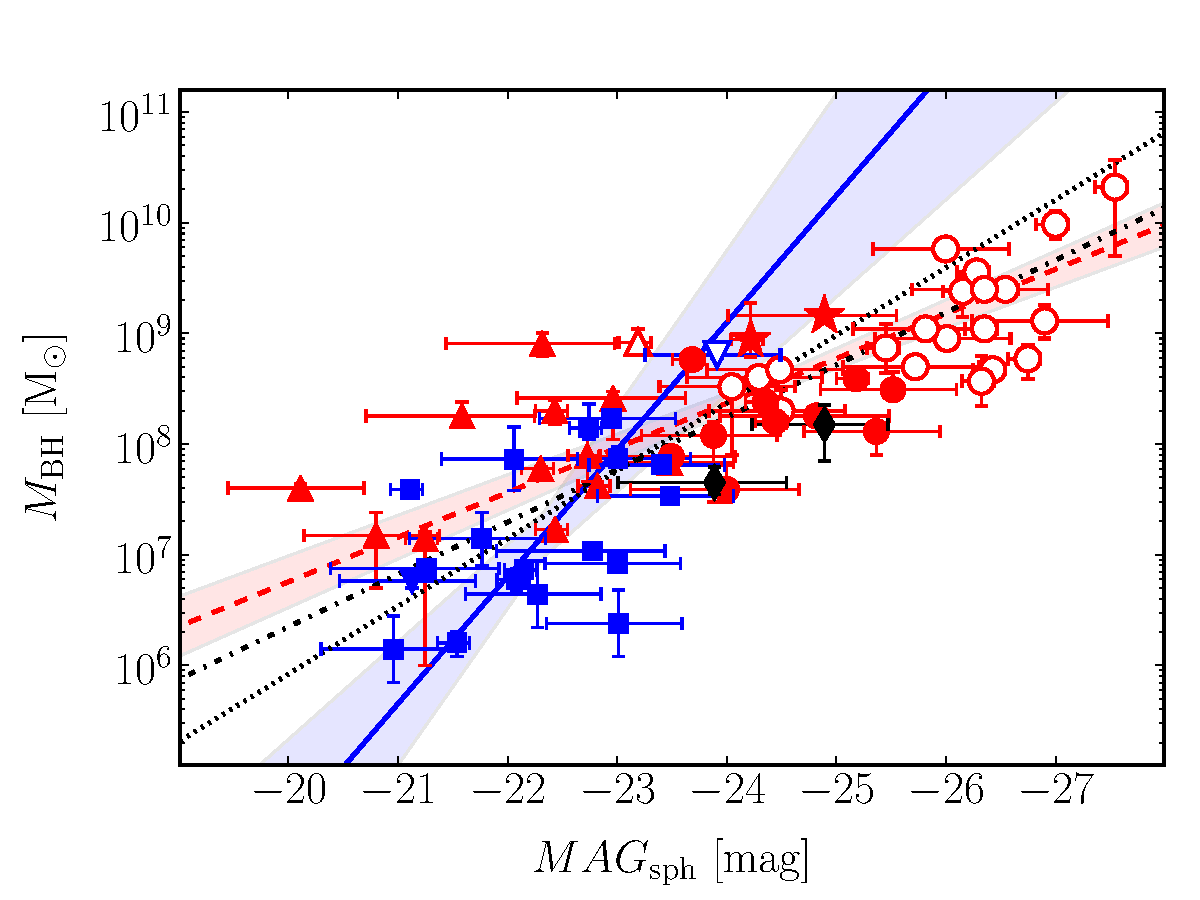
\includegraphics[width=\columnwidth]{images/mbh_vs_mag_sph.pdf}
\caption{Black hole mass against $3.6\rm~\mu m$ spheroid absolute magnitude. 
Symbols are coded according to the galaxy morphological type: red circle = elliptical, red star = elliptical/lenticular, 
red upward triangle = lenticular, blue downward triangle = lenticular/spiral, blue square = spiral, black diamond = merger. 
Empty symbols represent core-S\'ersic spheroids, whereas filled symbols are used for S\'ersic spheroids. 
The red dashed line indicates the BCES bisector linear regression for early-type galaxies (ellipticals+lenticulars), 
with the red shaded area denoting its $1\sigma$ uncertainty. 
The blue solid line shows the BCES bisector linear regression for spiral galaxies, 
with the blue shaded area denoting its $1\sigma$ uncertainty. 
The black dashed-dotted and dotted lines represent the BCES bisector linear regressions for core-S\'ersic and S\'ersic spheroids, respectively.}
\label{fig:mbhmagsph}
\end{center}
\end{figure}

\begin{figure}[h]
\begin{center}
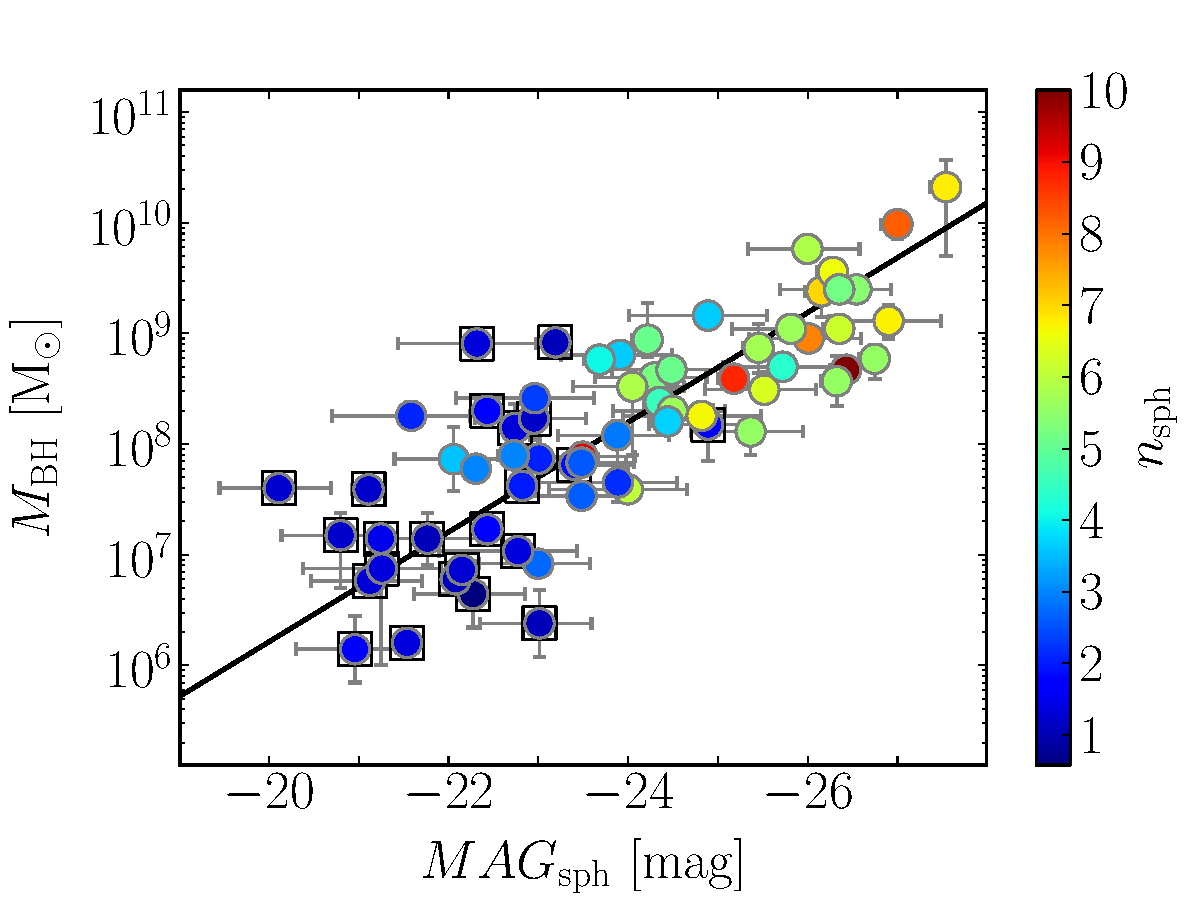
\includegraphics[width=\columnwidth]{images/mbh_vs_mag_sph_psb.pdf}
\caption{Black hole mass against $3.6\rm~\mu m$ spheroid absolute magnitude. 
Symbols are color coded according to the spheroid S\'ersic index $n_{\rm sph}$. 
Bulges with $n_{\rm sph}<2$, claimed by some to be pseudobulges, are marked with an empty square. 
The black solid line shows the BCES bisector linear regression for spheroids with $n_{\rm sph} \geq 2$. 
The inset displays, for all spheroids, the vertical offset 
from the correlation defined by spheroids with $n_{\rm sph} \geq 2$ only 
versus the spheroid S\'ersic index. 
The vertical dashed line corresponds to $n_{\rm sph} = 2$.
Bulges with $n_{\rm sph}<2$ are not randomly offset to lower black hole masses 
from the correlation traced by bulges with $n_{\rm sph} \geq 2$.}
\label{fig:pseudob}
\end{center}
\end{figure}

\begin{figure}[h]
\begin{center}
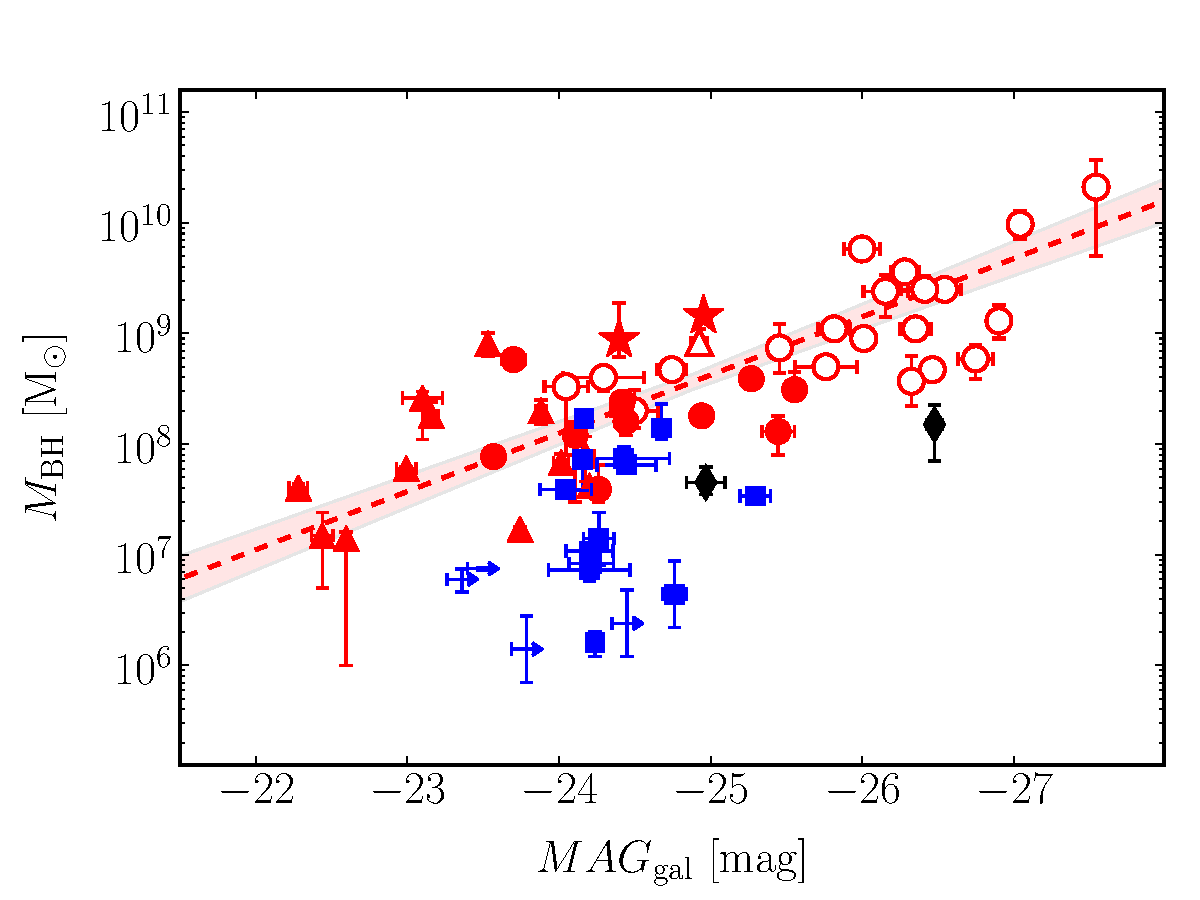
\includegraphics[width=\columnwidth]{images/mbh_vs_mag_tot.pdf}
\caption{Black hole mass against $3.6\rm~\mu m$ galaxy absolute magnitude. 
Symbols are coded as in Figure \ref{fig:mbhmagsph}.
Four spiral galaxies had their magnitudes overestimated and are shown as upper limits. 
}
\label{fig:mbhmaggal}
\end{center}
\end{figure}



\begin{figure}[h]
\begin{center}
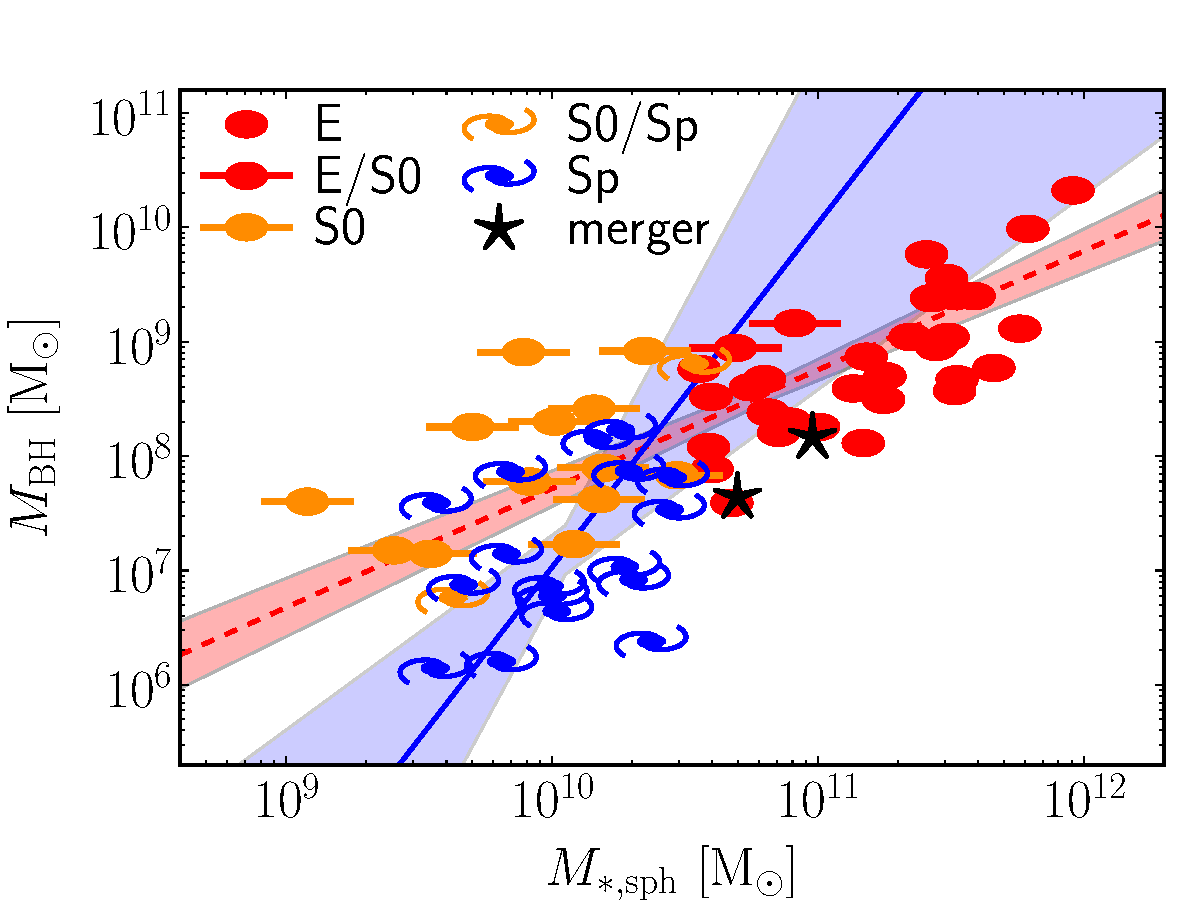
\includegraphics[width=\columnwidth]{images/mbh_vs_mass_sph.pdf}
\caption{Black hole mass against spheroid stellar mass. 
Symbols are coded according to the galaxy morphological type (red = E, orange = E/S0 and S0, blue = S0/Sp and Sp, black = merger).
The red dashed line indicates the BCES bisector linear regression for early-type galaxies (ellipticals+lenticulars), 
with the red shaded area denoting its $1\sigma$ uncertainty. 
The blue solid line shows the BCES bisector linear regression for spiral galaxies, 
with the blue shaded area denoting its $1\sigma$ uncertainty. }
\label{fig:mbhmasssph}
\end{center}
\end{figure}



\begin{table*}
\centering
\caption{Linear regression analysis. {\bf X0 is the average X of the subsample...}}
\begin{tabular}{llccccc}
\hline
\hline
{\bf Subsample (size)} & {\bf Regression} & $\boldsymbol \alpha$ & $\boldsymbol \beta$ & $\boldsymbol X_0$ & $\boldsymbol \epsilon$ & $\boldsymbol \Delta$ \\ 
\hline 
\\
 & \multicolumn{6}{l}{\emph{Black hole mass -- spheroid luminosity}} \\
 & \multicolumn{6}{l}{$\log[M_{\rm BH}/{\rm M_\odot}] = \alpha + \beta[(MAG_{\rm sph} - X_0)/{\rm mag}]$} \\ [0.5em]
All (66)               & BCES OLS$(Y|X)$   & $8.16 \pm 0.07$ & $-0.44 \pm 0.04$ & $-23.86$ & $-$ & $0.56$ \\
                       & BCES OLS$(X|Y)$   & $8.16 \pm 0.08$ & $-0.61 \pm 0.05$ & $-23.86$ & $-$ & $0.68$ \\
                       & BCES Bisector     & $8.16 \pm 0.07$ & $-0.52 \pm 0.04$ & $-23.86$ & $-$ & $0.60$ \\
                       & mFITEXY OLS$(Y|X)$ & $8.17^{+0.07}_{-0.06}$ & $-0.43^{+0.03}_{-0.03}$ & $-23.86$ & $0.49^{+0.06}_{-0.05}$ & $0.56$ \\
                       & mFITEXY OLS$(X|Y)$ & $8.15^{+0.07}_{-0.08}$ & $-0.61^{+0.05}_{-0.05}$ & $-23.86$ & $0.58^{+0.07}_{-0.06}$ & $0.67$ \\
                       & mFITEXY Bisector   & $8.16^{+0.07}_{-0.07}$ & $-0.51^{+0.04}_{-0.04}$ & $-23.86$ & $-$    & $0.60$ \\
                       & Kelly OLS$(Y|X)$  & $8.16 \pm 0.07$ & $-0.42 \pm 0.04$ & $-23.86$ & $0.51 \pm 0.06$ & $0.56$ \\
                       & Kelly OLS$(X|Y)$  & $8.16 \pm 0.09$ & $-0.60 \pm 0.06$ & $-23.86$ & $0.60 \pm 0.09$ & $0.67$ \\
                       & Kelly Bisector    & $8.16 \pm 0.08$ & $-0.51 \pm 0.09$ & $-23.86$ & $-$    & $0.59$ \\ [0.5em]

$n>2$ (43)             & BCES OLS$(Y|X)$   & $8.58 \pm 0.07$ & $-0.42 \pm 0.06$ & $-24.77$ & $-$ & $0.46$ \\
                       & BCES OLS$(X|Y)$   & $8.58 \pm 0.08$ & $-0.58 \pm 0.06$ & $-24.77$ & $-$ & $0.56$ \\
                       & BCES Bisector     & $8.58 \pm 0.07$ & $-0.50 \pm 0.05$ & $-24.77$ & $-$ & $0.49$ \\
                       & mFITEXY OLS$(Y|X)$ & $8.57^{+0.07}_{-0.06}$ & $-0.41^{+0.04}_{-0.04}$ & $-24.77$ & $0.38^{+0.06}_{-0.06}$ & $0.46$ \\
                       & mFITEXY OLS$(X|Y)$ & $8.56^{+0.08}_{-0.08}$ & $-0.57^{+0.06}_{-0.07}$ & $-24.77$ & $0.44^{+0.08}_{-0.11}$ & $0.55$ \\
                       & mFITEXY Bisector   & $8.57^{+0.07}_{-0.07}$ & $-0.49^{+0.05}_{-0.05}$ & $-24.77$ & $-$    & $0.49$ \\
                       & Kelly OLS$(Y|X)$  & $8.56 \pm 0.07$ & $-0.39 \pm 0.05$ & $-24.77$ & $0.40 \pm 0.06$ & $0.46$ \\
                       & Kelly OLS$(X|Y)$  & $8.55 \pm 0.09$ & $-0.57 \pm 0.08$ & $-24.77$ & $0.49 \pm 0.10$ & $0.55$ \\
                       & Kelly Bisector    & $8.55 \pm 0.08$ & $-0.5 \pm 0.1$ & $-24.77$ & $-$    & $0.49$ \\  [0.5em]
                   
Core-S\'ersic (22) & BCES OLS$(Y|X)$   & $9.06 \pm 0.09$ & $-0.3  \pm 0.1$  & $-25.73$ & $-$    & $0.42$ \\
                   & BCES OLS$(X|Y)$   & $9.1  \pm 0.1$  & $-0.6  \pm 0.1$  & $-25.73$ & $-$    & $0.61$ \\
                   & BCES Bisector     & $9.1  \pm 0.1$  & $-0.47 \pm 0.08$ & $-25.73$ & $-$    & $0.48$ \\
                   & mFITEXY OLS$(Y|X)$ & $9.06^{+0.09}_{-0.08}$ & $-0.26^{+0.07}_{-0.08}$ & $-25.73$ & $0.37^{+0.08}_{-0.06}$ & $0.42$ \\
                   & mFITEXY OLS$(X|Y)$ & $9.0^{+0.1}_{-0.1}$ & $-0.7^{+0.2}_{-0.3}$ & $-25.73$ & $0.61^{+0.14}_{-0.09}$ & $0.67$ \\
                   & mFITEXY Bisector   & $9.0^{+0.1}_{-0.1}$ & $-0.5^{+0.1}_{-0.2}$ & $-25.73$ & $-$    & $0.48$ \\
                   & Kelly OLS$(Y|X)$  & $9.0 \pm 0.1$ & $-0.24 \pm 0.09$ & $-25.73$ & $0.40 \pm 0.08$ & $0.42$ \\
                   & Kelly OLS$(X|Y)$  & $9.0 \pm 0.2$ & $-0.7 \pm 0.3$ & $-25.73$ & $0.68 \pm 0.30$ & $0.64$ \\
                   & Kelly Bisector    & $9.0 \pm 0.1$ & $-0.4 \pm 0.1$ & $-25.73$ & $-$    & $0.46$ \\ [0.5em]

S\'ersic (44) & BCES OLS$(Y|X)$   & $7.71 \pm 0.09$ & $-0.41 \pm 0.08$ & $-22.92$ & $-$    & $0.61$ \\
              & BCES OLS$(X|Y)$   & $7.7  \pm 0.1$  & $-0.9  \pm 0.2 $ & $-22.92$ & $-$    & $0.93$ \\
              & BCES Bisector     & $7.7  \pm 0.1$  & $-0.61 \pm 0.08$ & $-22.92$ & $-$    & $0.71$ \\
              & mFITEXY OLS$(Y|X)$ & $7.72^{+0.08}_{-0.08}$ & ${-0.41}^{+0.07}_{-0.07}$ & $-22.92$ & $0.54^{+0.09}_{-0.07}$ & $0.61$ \\
              & mFITEXY OLS$(X|Y)$ & $7.7^{+0.1}_{-0.1}$ & $-0.9^{+0.1}_{-0.2}$ & $-22.92$ & $0.77^{+0.13}_{-0.10}$ & $0.93$ \\
              & mFITEXY Bisector   & $7.7^{+0.1}_{-0.1}$ & $-0.61^{+0.09}_{-0.12}$ & $-22.92$ & $-$     & $0.71$ \\
              & Kelly OLS$(Y|X)$  & $7.73 \pm 0.09$ & $-0.41 \pm 0.08$ & $-22.92$ & $0.55 \pm 0.08$ & $0.61$ \\
              & Kelly OLS$(X|Y)$  & $7.7 \pm  0.1$ & $-0.9 \pm 0.2$ & $-22.92$ & $0.79 \pm  0.20$ & $0.93$ \\
              & Kelly Bisector    & $7.7 \pm 0.1$ & $-0.6 \pm 0.1$ & $-22.92$ & $-$    & $0.71$ \\ [0.5em]

%Ellipticals (E) (30)   & BCES OLS$(Y|X)$   & $8.80 \pm 0.07$ & $-0.53 \pm 0.09$ & $-25.45$ & $-$    & $0.42$ \\
%                      & BCES OLS$(X|Y)$   & $8.80 \pm 0.08$ & $-0.66 \pm 0.07$ & $-25.45$ & $-$    & $0.48$ \\
%                      & BCES Bisector     & $8.80 \pm 0.08$ & $-0.59 \pm 0.07$ & $-25.45$ & $-$    & $0.44$ \\
%                      & FITEXY OLS$(Y|X)$ & $8.81^{+0.07}_{-0.07}$ & $-0.44^{+0.06}_{-0.07}$ & $-25.45$ & $0.33$     & $0.40$ \\
%                      & FITEXY OLS$(X|Y)$ & $8.78^{+0.09}_{-0.09}$ & $-0.7^{+0.1}_{-0.1}$    & $-25.45$ & $0.60$     & $0.50$\\
%                      & FITEXY Bisector   & $8.80^{+0.08}_{-0.08}$ & $-0.56^{+0.08}_{-0.10}$ & $-25.45$ & $-$        & $0.43$ \\
%
%Lenticulars (S0) (13)  & BCES OLS$(Y|X)$   & $7.9 \pm 0.1$ & $-0.4 \pm 0.2$ & $-22.19$ & $-$    & $0.56$ \\
%                      & BCES OLS$(X|Y)$   & $7.9 \pm 0.3$ & $-1.1 \pm 0.5$ & $-22.19$ & $-$    & $1.01$ \\
%                      & BCES Bisector     & $7.9 \pm 0.2$ & $-0.7 \pm 0.2$ & $-22.19$ & $-$    & $0.69$ \\
%                      & FITEXY OLS$(Y|X)$ & $7.9^{+0.2}_{-0.1}$ & $-0.3^{+0.2}_{-0.2}$ & $-22.19$ & $0.51$     & $0.56$ \\
%                      & FITEXY OLS$(X|Y)$ & $7.8^{+0.3}_{-0.4}$ & $-1.3^{+0.4}_{-1.3}$ & $-22.19$ & $0.71$     & $1.20$\\
%                      & FITEXY Bisector   & $7.9^{+0.2}_{-0.3}$ & $-0.7^{+0.3}_{-0.4}$ & $-22.19$ & $-$        & $0.71$ \\
%
{\bf Early-type (E+S0)} (45) & BCES OLS$(Y|X)$    & $8.56 \pm 0.07$ & $-0.33 \pm 0.04$ & $-24.47$ & $-$    & $0.46$ \\
                             & BCES OLS$(X|Y)$    & $8.56 \pm 0.08$ & $-0.48 \pm 0.05$ & $-24.47$ & $-$    & $0.55$ \\
                             & {\bf BCES Bisector}& $\boldsymbol{8.56 \pm 0.07}$ & $\boldsymbol{-0.40 \pm 0.04}$ & $\boldsymbol{-24.47}$ & $-$    & $\boldsymbol{0.49}$ \\
                             & mFITEXY OLS$(Y|X)$ & $8.56^{+0.06}_{-0.06}$ & $-0.32^{+0.03}_{-0.04}$ & $-24.47$ & $0.40^{+0.06}_{-0.05}$ & $0.46$ \\
                             & mFITEXY OLS$(X|Y)$ & $8.54^{+0.08}_{-0.08}$ & $-0.49^{+0.05}_{-0.06}$ & $-24.47$ & $0.49^{+0.08}_{-0.06}$ & $0.57$\\
                             & mFITEXY Bisector   & $8.55^{+0.07}_{-0.07}$ & $-0.41^{+0.04}_{-0.05}$ & $-24.47$ & $-$    & $0.49$ \\
                             & Kelly OLS$(Y|X)$  & $8.55 \pm 0.07$ & $-0.32 \pm 0.04$ & $-24.47$ & $0.41 \pm 0.06$ & $0.46$ \\
                             & Kelly OLS$(X|Y)$  & $8.55 \pm 0.09$ & $-0.48 \pm 0.06$ & $-24.47$ & $0.51 \pm 0.10$ & $0.56$ \\
                             & Kelly Bisector    & $8.55 \pm 0.08$ & $-0.40 \pm 0.09$ & $-24.47$ & $-$    & $0.49$ \\ [0.5em]

{\bf Late-type (Sp)} (17) & BCES OLS$(Y|X)$    & $7.2 \pm 0.2$ & $-0.8 \pm 0.4$ & $-22.33$ & $-$    & $0.70$ \\
                          & BCES OLS$(X|Y)$    & $7.2 \pm 0.3$ & $-1.7 \pm 0.7$ & $-22.33$ & $-$    & $1.26$ \\
                          & {\bf BCES Bisector}& $\boldsymbol{7.2 \pm 0.2}$ & $\boldsymbol{-1.1 \pm 0.3}$ & $\boldsymbol{-22.33}$ & $-$    & $\boldsymbol{0.88}$ \\
                          & mFITEXY OLS$(Y|X)$ & $7.2^{+0.1}_{-0.1}$ & $-0.5^{+0.2}_{-0.2}$ & $-22.33$ & $0.55^{+0.15}_{-0.10}$ & $0.62$ \\
                          & mFITEXY OLS$(X|Y)$ & $7.4^{+0.5}_{-0.3}$ & $-2.0^{+0.7}_{-2.4}$ & $-22.33$ & $1.08^{+0.40}_{-0.24}$ & $1.50$ \\
                          & mFITEXY Bisector   & $7.3^{+0.4}_{-0.3}$ & $-1.0^{+0.3}_{-0.5}$ & $-22.33$ & $-$    & $0.82$ \\
                          & Kelly OLS$(Y|X)$  & $7.2 \pm 0.2$ & $-0.5 \pm 0.3$ & $-22.33$ & $0.64 \pm 0.16$ & $0.62$ \\
                          & Kelly OLS$(X|Y)$  & $7.3 \pm 0.4$ & $-1.9 \pm 1.2$ & $-22.33$ & $1.3 \pm 0.9$ & $1.4$ \\
                          & Kelly Bisector    & $7.3 \pm 0.3$ & $-0.9 \pm 0.5$ & $-22.33$ & $-$    & $0.78$ \\

\hline 
\hline
\end{tabular}
\label{tab:lreg} 
\end{table*}

\begin{table*}
\centering
\caption{Linear regression analysis. {\bf X0 is the average X of the subsample...}}
\begin{tabular}{llccccc}
\hline
\hline
{\bf Subsample (size)} & {\bf Regression} & $\boldsymbol \alpha$ & $\boldsymbol \beta$ & $\boldsymbol X_0$ & $\boldsymbol \epsilon$ & $\boldsymbol \Delta$ \\ 
\hline 
\\
 & \multicolumn{6}{l}{\emph{Black hole mass -- galaxy luminosity}} \\
  & \multicolumn{6}{l}{$\log[M_{\rm BH}/{\rm M_\odot}] = \alpha + \beta[(MAG_{\rm gal} - X_0)/{\rm mag}]$} \\ [0.5em]
 All (62)		& BCES OLS$(Y|X)$   & $8.26 \pm 0.08$ & $-0.49 \pm 0.06$ & $-24.78$ & $-$ & $0.64$ \\
 			& BCES OLS$(X|Y)$   & $8.3 \pm 0.1$   & $-1.0 \pm 0.1$   & $-24.78$ & $-$ & $0.92$ \\
 			& BCES Bisector     & $8.26 \pm 0.09$ & $-0.72 \pm 0.07$ & $-24.78$ & $-$ & $0.71$ \\
 			& mFITEXY OLS$(Y|X)$ & $8.26^{+0.08}_{-0.08}$ & $-0.49^{+0.06}_{-0.07}$ & $-24.78$ & $0.61^{+0.07}_{-0.05}$ & $0.64$ \\
 			& mFITEXY OLS$(X|Y)$ & $8.3^{+0.1}_{-0.1}$    & $-1.0^{+0.1}_{-0.2}$	& $-24.78$ & $0.88^{+0.10}_{-0.08}$ & $0.93$ \\
 			& mFITEXY Bisector   & $8.3^{+0.1}_{-0.1}$    & $-0.72^{+0.09}_{-0.10}$ & $-24.78$ & $-$    & $0.71$ \\
 			& Kelly OLS$(Y|X)$  & $8.26 \pm 0.08$ & $-0.49 \pm 0.07$ & $-24.78$ & $0.63 \pm 0.07$ & $0.64$ \\
 			& Kelly OLS$(X|Y)$  & $8.3 \pm 0.1$ & $-1.0 \pm 0.1$ & $-24.78$ & $0.91 \pm 0.17$ & $0.93$ \\
 			& Kelly Bisector    & $8.3 \pm 0.1$ & $-0.7 \pm 0.1$ & $-24.78$ & $-$    & $0.71$ \\ [0.5em]

 Early-type (E+S0) (45) & BCES OLS$(Y|X)$   & $8.56 \pm 0.06$ & $-0.43 \pm 0.05$ & $-24.88$ & $-$ & $0.45$ \\
 			& BCES OLS$(X|Y)$   & $8.56 \pm 0.08$ & $-0.63 \pm 0.05$ & $-24.88$ & $-$ & $0.53$ \\
 			& BCES Bisector     & $8.56 \pm 0.07$ & $-0.53 \pm 0.04$ & $-24.88$ & $-$ & $0.47$ \\
 			& mFITEXY OLS$(Y|X)$ & $8.56^{+0.06}_{-0.06}$ & $-0.42^{+0.05}_{-0.05}$ & $-24.88$ & $0.41^{+0.06}_{-0.05}$ & $0.45$ \\
 			& mFITEXY OLS$(X|Y)$ & $8.56^{+0.08}_{-0.08}$ & $-0.66^{+0.06}_{-0.08}$ & $-24.88$ & $0.51^{+0.07}_{-0.06}$ & $0.55$ \\
 			& mFITEXY Bisector   & $8.56^{+0.07}_{-0.07}$ & $-0.54^{+0.06}_{-0.06}$ & $-24.88$ & $-$    & $0.47$ \\
 			& Kelly OLS$(Y|X)$  & $8.56 \pm 0.07$ & $-0.42 \pm 0.06$ & $-24.88$ & $0.43 \pm 0.06$ & $0.45$ \\
 			& Kelly OLS$(X|Y)$  & $8.56 \pm 0.09$ & $-0.65 \pm 0.08$ & $-24.88$ & $0.53 \pm 0.10$ & $0.54$ \\
 			& Kelly Bisector    & $8.56 \pm 0.08$ & $-0.5 \pm 0.1$ & $-24.88$ & $-$    & $0.47$ \\

%All (62)               & BCES OLS$(Y|X)$   & $$ & $$ & $$ & $-$ & $$ \\
%                       & BCES OLS$(X|Y)$   & $$ & $$ & $$ & $-$ & $$ \\
%                       & BCES Bisector     & $$ & $$ & $$ & $-$ & $$ \\
%                       & FITEXY OLS$(Y|X)$ & $$ & $$ & $$ & $$ & $$ \\
%                       & FITEXY OLS$(X|Y)$ & $$ & $$ & $$ & $$ & $$ \\
%                       & FITEXY Bisector   & $$ & $$ & $$ & $-$    & $$ \\
%                       & Kelly OLS$(Y|X)$  & $$ & $$ & $$ & $$ & $$ \\
%                       & Kelly OLS$(X|Y)$  & $$ & $$ & $$ & $$ & $$ \\
%                       & Kelly Bisector    & $$ & $$ & $$ & $-$    & $$ \\

\hline 
\\
 & \multicolumn{6}{l}{\emph{Black hole mass -- spheroid stellar mass}} \\
  & \multicolumn{6}{l}{$\log[M_{\rm BH}/{\rm M_\odot}] = \alpha + \beta \log[(M_{\rm *,sph} - X_0)/{\rm M_\odot}]$} \\ [0.5em]
{\bf Early-type (E+S0)} (45)  & BCES OLS$(Y|X)$    & $8.56 \pm 0.07$ & $0.8 \pm 0.1$ & $10.81$ & $-$ & $0.48$ \\
                              & BCES OLS$(X|Y)$    & $8.56 \pm 0.08$ & $1.3 \pm 0.1$ & $10.81$ & $-$ & $0.59$ \\
                              & {\bf BCES Bisector}& $\boldsymbol{8.56 \pm 0.07}$ & $\boldsymbol{1.0 \pm 0.1}$ & $\boldsymbol{10.81}$ & $-$ & $\boldsymbol{0.51}$ \\
                              & mFITEXY OLS$(Y|X)$  & $8.56^{+0.06}_{-0.07}$ & $0.8^{+0.1}_{-0.1}$ & $10.81$ & $0.42^{+0.06}_{-0.05}$ & $0.48$ \\
                              & mFITEXY OLS$(X|Y)$  & $8.54^{+0.09}_{-0.08}$ & $1.3^{+0.2}_{-0.1}$ & $10.81$ & $0.53^{+0.08}_{-0.07}$ & $0.61$ \\
                              & mFITEXY Bisector    & $8.55^{+0.07}_{-0.08}$ & $1.0^{+0.1}_{-0.1}$ & $10.81$ & $-$                    & $0.51$ \\
                              & Kelly OLS$(Y|X)$  & $8.55 \pm 0.07$ & $0.8 \pm 0.1$ & $10.81$ & $0.43 \pm 0.06$ & $0.48$ \\
                              & Kelly OLS$(X|Y)$  & $8.55 \pm 0.09$ & $1.3 \pm 0.2$ & $10.81$ & $0.54 \pm 0.11$ & $0.59$ \\
                              & Kelly Bisector    & $8.55 \pm 0.08$ & $1.0 \pm 0.2$ & $10.81$ & $-$    & $0.51$ \\ [0.5em]

{\bf Late-type (Sp)} (17)    & BCES OLS$(Y|X)$    & $7.2 \pm 0.2$ & $1.9 \pm 1.5$ & $10.05$ & $-$ & $0.74$ \\ 
                             & BCES OLS$(X|Y)$    & $7.2 \pm 0.4$ & $5.9 \pm 3.4$ & $10.05$ & $-$ & $1.70$ \\
                             & {\bf BCES Bisector}& $\boldsymbol{7.2 \pm 0.2}$ & $\boldsymbol{3.0 \pm 1.3}$ & $\boldsymbol{10.05}$ & $-$ & $\boldsymbol{0.94}$ \\
                             & mFITEXY OLS$(Y|X)$  & $7.2^{+0.1}_{-0.2}$ & $1.2^{+0.7}_{-0.6}$ & $10.05$ & $0.59^{+0.16}_{-0.11}$ & $0.66$ \\
                             & mFITEXY OLS$(X|Y)$  & $7.4^{+1.5}_{-0.5}$ & $7.1^{+26.3}_{-3.0}$ & $10.05$ & $1.49^{+0.57}_{-0.35}$ & $2.08$ \\
                             & mFITEXY Bisector    & $7.2^{+1.0}_{-0.4}$ & $2.3^{+1.7}_{-1.0}$ & $10.05$ & $-$    & $0.79$ \\
                             & Kelly OLS$(Y|X)$  & $7.2 \pm 0.2$ & $0.9 \pm 0.9$ & $10.05$ & $0.67 \pm 0.16$ & $0.65$ \\
                             & \textcolor{red}{Kelly OLS$(X|Y)$}  & $7.4 \pm 0.6$ & $7.0 \pm 6.6$ & $10.05$ & $1.83 \pm 1.82$ & $2.04$ \\
                             & \textcolor{red}{Kelly Bisector}    & $7.3 \pm 0.5$ & $1.9 \pm 203.0$ & $10.05$ & $-$    & $0.74$ \\
                  
\hline 
\hline
\end{tabular}
\label{tab:lreg} 
\end{table*}


\section{Analysis}
\label{sec:anal}
We performed a linear regression analysis of the $M_{\rm BH} - L_{\rm sph}$, $M_{\rm BH} - M_{\rm *,sph}$ and $M_{\rm BH} - L_{\rm gal}$ diagrams 
using the BCES code from \cite{akritasbershady1996}. 
We also repeated the analysis with the FITEXY routine \citep{press1992}, modified by \cite{tremaine2002}, 
and the Bayesian estimator {\tt linmix\_err} \citep{linmixerr}. 
Although all these three linear regression routines account for the intrinsic scatter, 
only the last two allow to quantify it.
%Because the BCES routine {\bf AL: did you wanna write (correctly) this sentence for me please? 
%can give biased results (wrong slope) when the scatter is comparable to the range of the data},
%we checked that the best-fit parameters obtained with the BCES code were consistent with those output by the modified FITEXY code.
In Table \ref{tab:lreg}, we report the BCES, modified FITEXY and {\tt linmix\_err} linear regressions, both symmetrical and non-symmetrical, 
for S\'ersic/core-S\'ersic galaxies and for different galaxy morphological types (elliptical/lenticular, spiral).
Symmetrical regressions are meant to be compared with theoretical expectations, 
whereas non-symmetrical Ordinary Least Squares $(Y|X)$ regressions -- 
since they minimize the scatter in the vertical direction -- 
can be used to predict black hole masses.

\section{Results and discussion}
\label{sec:res}

\subsection{Black hole mass -- spheroid luminosity}
We show the $M_{\rm BH} - L_{\rm sph}$ diagram in Figure \ref{fig:mbhmagsph}. \\
S\'ersic and core-S\'ersic spheroids have slopes consistent with each other (within their $1\sigma$ uncertainties), 
in disagreement with the findings of GS13. 
The slope that we obtained for core-S\'ersic spheroids ($M_{\rm BH} \propto L_{\rm sph}^{1.2 \pm 0.2}$) 
is consistent with the slope reported by GS13 in the $K_s$-band ($M_{\rm BH} \propto L_{\rm sph}^{1.1 \pm 0.2}$). 
Instead, the slope that we determined for S\'ersic spheroids ($M_{\rm BH} \propto L_{\rm sph}^{1.5 \pm 0.2}$) 
is significantly shallower than that found by GS13 ($M_{\rm BH} \propto L_{\rm sph}^{2.7 \pm 0.5}$). 
Although the S\'ersic/core-S\'ersic classification used by GS13 slightly differs\footnote{which galaxies?} from the classification used here, 
the main cause of such inconsistency is that the bulge-to-total ratios obtained from our galaxy decompositions 
are different from those assumed by GS13 to convert galaxy luminosities into bulge luminosities.
Our bulge-to-total ratios for low-luminosity S\'ersic spheroids ($MAG_{\rm sph} \gtrsim -22 \rm~mag$) 
are smaller than those used by GS13. 
The host galaxies of such bulges are late-type, spiral galaxies, 
which typically present a complex morphology (bars, double bars, embedded disks, nuclear components, etc).
Our sophisticated galaxy models account for the extra components, 
while the bulge-to-total ratios of GS13 were derived from simple bulge/disk decompositions 
which overestimated the bulge luminosity.
This results in our bulge magnitudes being on average $\sim$$1\rm~mag$ fainter.
On the other side, our bulge-to-total ratios for high-luminosity S\'ersic spheroids ($MAG_{\rm sph} \lesssim -24 \rm~mag$) 
are on average larger than those adopted by GS13.
In this case, the host systems are early-type elliptical/lenticular galaxies that feature intermediate-scale disks\footnote{explain}.
Past bulge/disk decompositions failed to correctly identify the extent of such disks and treated them as large-scale disks, 
thus underestimating the bulge luminosity.
The magnitudes that we obtained for such spheroids are on average $\sim$$1\rm~mag$ brighter. \\
We have seen that the change in slope of the $M_{\rm BH} - L_{\rm sph}$ correlation -- 
which is expected for consistency with other scaling relations 
(a single power-law $M_{\rm BH} - \sigma$ correlation and a double power-law $L_{\rm sph} - \sigma$ correlation) -- 
cannot be attributed to the division between the two populations of S\'ersic and core-S\'ersic spheroids.
We now test a new hypothesis, that is to say the change in slope is to be ascribed to the different formation mechanisms of early- and late-type galaxies. 
If this hypothesis is correct, 
the spheroids of early-type (elliptical and lenticular) galaxies will follow $M_{\rm BH} \propto L_{\rm sph}^{\sim 1}$, 
whereas the spheroids of late-type (spiral) galaxies will have $M_{\rm BH} \propto L_{\rm sph}^{\sim 2.5}$.
First, we checked that elliptical and lenticular galaxies, taken separately, have slopes consistent with each other, 
and thus, taken together, they define a single \emph{red sequence} in the $M_{\rm BH} - L_{\rm sph}$ diagram. 
We then fit the bulges of early- and late-type galaxies with two separate log-linear regressions, 
and obtained $M_{\rm BH} \propto L_{\rm sph}^{1 \pm 0.1}$ and $M_{\rm BH} \propto L_{\rm sph}^{2.75 \pm 0.75}$ respectively, 
in excellent agreement with the theoretical expectations of our hypothesis.
%{\bf vertical scatter along the early type sequence is constant? if 2 overmassive bhs removed, what happens?}
{\bf AL, can you pls write this: 
Remember also Ewan's remark about the unsuitability of the Pearson and Spearman correlation coefficients because 
they do not take into account the error bars on our data - 
so don't include those simple coefficients.  
Actually, it would be worth pointing out to readers that a visual inspection of the plotted data requires 
the viewer to take into account the error bars when judging-by-eye the strength of a correlation. 
Maybe then mention in the following sentence that this is why the correlation coefficients are not applicable here. }

\subsection{Pseudo- versus classical bulges}
Current views distinguish between classical bulges, which are considered to be spheroidal, pressure-supported systems, 
formed through violent processes, such as hierarchical clustering via minor mergers, 
and pseudo-bulges, thought to be disk-like, rotation-supported systems, 
built from secular evolution processes, such as instabilities of their surrounding disk or bar. 
Pseudo-bulges are notoriously hard to identify \citep{graham2013review,graham2014review,graham2015pseudo,graham2015review}.
For example, mergers can create bulges that rotate (e.g.~\citealt{bekki2010,keselmannusser2012}), 
and bars can spin-up classical bulges (e.g.~\citealt{saha2012}), 
thus rotation is not a definitive signature of a pseudobulge. 
Furthermore, many galaxies host both a pseudo- and a classical bulge (e.g.~\citealt{erwin2003,erwin2015,athanassoula2005,Gadotti2009,
macarthur2009,dosanjosdasilva2013,seidel2015}). 
In the recent literature, pseudo- and classical bulges have been frequently told apart by means of a divide at a 
S\'ersic index of $n_{\rm sph}=2$ (e.g.~\citealt{fisherdrory2010}), 
although, from a selection of hundreds of disc galaxies imaged in the $K$-band, 
\cite{grahamworley2008} observed no such bimodality in the bulge S\'ersic indices. 
While pseudo-bulges are expected to have exponential-like surface brightness profiles ($n_{\rm sph} \simeq 1$), 
being disky components that formed from their surrounding exponential disks 
(e.g.~\citealt{bardeen1975,hohl1975,combessanders1981,combes1990,pfennigerfriedli1991}), 
it has been shown that mergers can create bulges with $n_{\rm sph}<2$
(e.g.~\citealt{elichemoral2011,scannapieco2011,querejeta2015}), 
just as low-luminosity elliptical galaxies (not built from the secular evolution of a disk)
are well known to have $n_{\rm sph}<2$ and even $n_{\rm sph}<1$ (e.g.~\citealt{davies1988,youngcurrie1994}). \\
\cite{sani2011} reported that pseudo-bulges -- which they labelled as such according to the $n_{\rm sph}<2$ criterion -- 
with low black hole masses ($M_{\rm BH} < 10^7\rm~M_\odot$) are significantly displaced from the correlation 
traced by classical bulges. 
In Figure \ref{fig:pseudob}, we show the distribution of spheroid S\'ersic indices\footnote{The spheroid S\'ersic indices 
are taken from our one-dimensional fits of the galaxy major-axis surface brightness profiles (\emph{Paper I}).} 
in the $M_{\rm BH} - L_{\rm sph}$ diagram.
Our aim is to check whether $n_{\rm sph}<2$ bulges 
are offset to lower black hole masses from the correlation defined by $n_{\rm sph}>2$ bulges. 
To do this, we fit a symmetrical linear regression to the bulges that have $n_{\rm sph}>2$ 
and we compute the vertical offset of all bulges from the regression. 
In the inset of Figure \ref{fig:pseudob}, we plot the vertical offset against $n_{\rm sph}$. 
From a visual inspection, bulges with $n_{\rm sph}<2$ do not appear to be offset from the correlation traced by bulges with $n_{\rm sph}>2$.


\subsection{Black hole mass -- galaxy luminosity}
Figure \ref{fig:mbhmaggal} illustrates the $M_{\rm BH} - L_{\rm gal}$ diagram.
Four spiral galaxies had their total luminosities underestimated (see Section \ref{sec:data}) 
and thus are not included in the linear regression analysis. 
Upon analyzing a sample of 35 galaxies, among which only four were classified as spiral galaxies, 
\cite{lasker2014anal} claimed that the $M_{\rm BH} - L_{\rm sph}$ and $M_{\rm BH} - L_{\rm gal}$ relations, 
which they fit with a single power-law, have consistent intrinsic scatter.
Here, instead, thanks to our double-sized galaxy sample that includes 17 spiral galaxies, 
we show that the claim made by \cite{lasker2014anal} is valid only for early-type galaxies. 
The $M_{\rm BH} - L_{\rm sph}$ correlation for all galaxies, irrespective of their morphological type, 
has intrinsic scatter $\epsilon_{(Y|X)} = 0.51 \pm 0.06\rm~dex$ (direct linear regression) 
and $\epsilon_{(X|Y)} = 0.60 \pm 0.09\rm~dex$ (inverse linear regression), 
whereas the $M_{\rm BH} - L_{\rm gal}$ correlation for all galaxies has $\epsilon_{(Y|X)} = 0.63 \pm 0.07\rm~dex$ 
and $\epsilon_{(X|Y)} = 0.91 \pm 0.17\rm~dex$.
When considering only early-type galaxies, 
we find that the $M_{\rm BH} - L_{\rm sph}$ and $M_{\rm BH} - L_{\rm gal}$ relations have the same level of intrinsic scatter 
($\epsilon_{(Y|X)} = 0.41 \pm 0.06\rm~dex$ and $\epsilon_{(X|Y)} = 0.51 \pm 0.10\rm~dex$ 
against $\epsilon_{(Y|X)} = 0.43 \pm 0.06\rm~dex$ and $\epsilon_{(X|Y)} = 0.53 \pm 0.10\rm~dex$).
{\bf We point out here that this result does not strongly depend on the value that we assumed for the uncertainty of galaxy magnitudes (0.25). 
In fact, we tested different values and found that we need $error >= 0.7 mag$ to say that gal lum has smaller intrinsic scatter.

From the observer's perspective, measuring galaxy luminosities is obviously easier and faster 
than performing galaxy decompositions to obtain bulge luminosities. 
This, combined with the results from our analysis, suggests that one should prefer the galaxy luminosity over the bulge luminosity 
to predict black hole masses in a sample of elliptical and lenticular galaxies only.


\subsection{Black hole mass -- spheroid stellar mass}
Finally, we present the $M_{\rm BH} - M_{\rm *,sph}$ diagram in Figure \ref{fig:mbhmasssph}.

relations
agns consistent w spirals, but analysis deferred to other paper
cubic growth


\section{Conclusions}
\label{sec:concl}
ngc0524 outlier, n1332 non outlier


\acknowledgments
GS warmly thanks Luca Cortese, Elisabete Lima Da Cunha and Gonzalo Diaz for useful discussion. \\
% referee thank you!!
This research was supported by Australian Research Council funding through grants
DP110103509 and FT110100263.
This work is based on observations made with the IRAC instrument \citep{fazio2004IRAC} 
on-board the Spitzer Space Telescope, 
which is operated by the Jet Propulsion Laboratory, 
California Institute of Technology under a contract with NASA.
This research has made use of the GOLDMine database \citep{goldmine} and the NASA/IPAC Extragalactic Database (NED) 
which is operated by the Jet Propulsion Laboratory, California Institute of Technology, 
under contract with the National Aeronautics and Space Administration. 
The BCES routine \citep{akritasbershady1996} was run via the python module 
written by Rodrigo Nemmen \citep{nemmen2012}, which is available at {\url https://github.com/rsnemmen/BCES}.

\bibliography{/Users/gsavorgnan/Dropbox_notsync/giulia_e_basta/Literature/SMBHbibliography}


\clearpage


\end{document}

